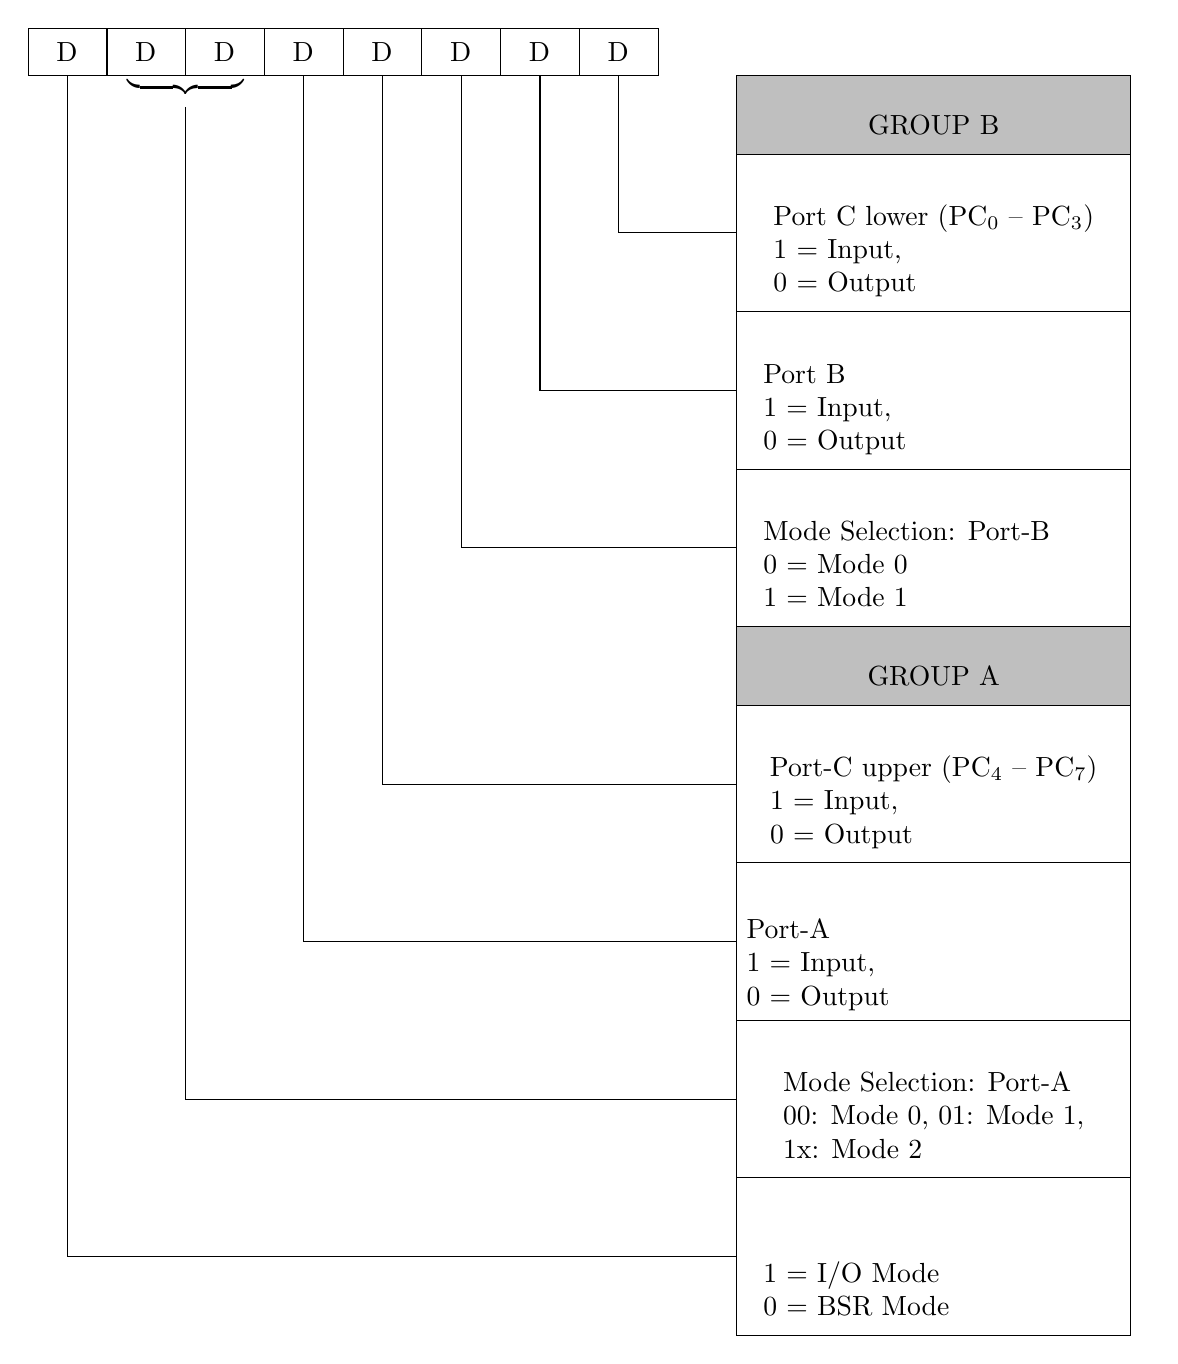
\begin{tikzpicture}
  \foreach \x in {1,...,8}
  {
    \FPeval{\lbl}{clip(8-\x)}
    \draw (\x,16) rectangle (\x+1,16.6) ;
    \draw (\x+0.5,16) node[anchor=south] {D$_{\lbl}$} ;
  }
  \foreach \y in {0,2,4,6}
  {
    \draw (10,\y) rectangle (15,\y+2) ;
  }
  \draw[fill=gray!50!white] (10,8) rectangle (15,9) ;
  \foreach \y in {9,11,13}
  {
    \draw (10,\y) rectangle (15,\y+2) ;
  }
  \draw[fill=gray!50!white] (10,15) rectangle (15,16) ;
  \draw (10,0) node[above right] {
    \begin{tabular}{l}
      1 = I/O Mode \\
      0 = BSR Mode
    \end{tabular}

  } ;
  \draw (12.5,2) node[anchor=south] {
    \begin{tabular}{l}
      Mode Selection: Port-A \\
      00: Mode 0, 01: Mode 1, \\
      1x: Mode 2
    \end{tabular}
  } ;
  \draw (10,4) node[above right] {
    \parbox[t]{5cm}{
      Port-A \\
      1 = Input, \\
      0 = Output
    }
  } ;
  \draw (12.5,6) node[anchor=south] {
    \begin{tabular}{l}
      Port-C upper (PC$_{4}$ -- PC$_{7}$) \\
      1 = Input, \\
      0 = Output
    \end{tabular}
  } ;
  \draw (12.5,8) node[anchor=south] {
    \begin{tabular}{l}
      GROUP A
    \end{tabular}
  } ;
  \draw (10,9) node[above right] {
    \begin{tabular}{l}
      Mode Selection: Port-B \\
      0 = Mode 0\\
      1 = Mode 1
    \end{tabular}
  } ;
  \draw (10,11) node[above right] {
    \begin{tabular}{l}
      Port B \\
      1 = Input, \\
      0 = Output
    \end{tabular}
  } ;
  \draw (12.5,13) node[anchor=south] {
    \begin{tabular}{l}
      Port C lower (PC$_{0}$ -- PC$_{3}$) \\
      1 = Input, \\
      0 = Output
    \end{tabular}
  } ;
  \draw (12.5,15) node[anchor=south] {
    \begin{tabular}{l}
      GROUP B
    \end{tabular}
  } ;
  \draw (1.5,16) |- (10,1) ;
  \draw (3,15.6)node[above]{$\underbrace{\phantom{aaaaaaaa}}$} to (3,3) to  (10,3) ;
  \draw (4.5,16) |- (10,5) ;
  \draw (5.5,16) |- (10,7) ;
  \draw (6.5,16) |- (10,10) ;
  \draw (7.5,16) |- (10,12) ;
  \draw (8.5,16) |- (10,14) ;
\end{tikzpicture}
